\chapter{DCM for Cross Spectral Densities: Anaesthesia Depth in Rodent Data\label{Chap:data:dcm_csd}}

\section{Overview}

This chapter describes the analysis of a 2-channel Local Field Potential (LFPs) data set using dynamic causal modelling. The LFPs were recorded from a single rodent using intracranial electrodes \cite{dcm_ssr_anaesthesia}. We thank Marc Tittgemeyer for providing us with this data. The theory behind DCM for cross spectral densities (DCM-CSD) is described in \cite{Friston2012439}. This DCM is a generalization of DCM for Steady State Responses to the complex domain \cite{dcm_ssr}. The generative model now reports coherence and signal covariance as well as complex spectral densities (from which the former are derived).

We measured local field potentials from primary (A1) and secondary auditory (A2) cortex in a rodent following the application of four different doses of the anaesthetic agent Isoflurane; 1.4, 1.8, 2.4 and 2.8\%. The rodent was presented with a white noise auditory input for several minutes at each anaesthetised level and time series recordings were obtained for the entire epoch. We performed a DCM analysis to ask whether changes in neuronal activity induced by increasing levels of Isoflurane are best accounted for by \emph{either} extrinsic \emph{or} intrinsic changes in connectivity.

We demonstrate in this chapter the consistency of the model comparison and conditional parameter estimates across different population models. In particular we modeled the CSD as the output of a two region network comprising either ``CMC'' or ``NMDA'' -- type neural mass models.  


The CMC-type neural mass model comprises four subpopulations. It is a refinement of the Jansen and Rit convolution models that explicitly accommodates the neuronal sources of forward and backward connections in cortical hierarchies \cite{Bastos2012}. These are distinct superficial and deep pyramidal cell populations respectively that, crucially, may exhibit different spectral outputs. The CMC thus utilizes different types of subpopulations as the source of forward and backward connections. For the forward connections superficial pyramidal cells excite stellate cells and deep pyramidal neurons, while the backward connections inhibit superficial pyramidal cells and inhibitory interneurons (see \texttt{spm\_fx\_cmc}).  From the graphical user interface trial specific effects can be selected for extrinsic connections or intrinsic connections, for the CMC case the intrinsic connection that is modulated is an inhibitory gain parameter on superficial pyramidal cells. The smaller this value, the greater the gain on this cell population due to the modulation. 

The NMDA model uses an architecture comprising three subpopulations, each assigned to a particular cortical layer. An inhibitory interneuron subpopulation occupies agranular layers. This receives inputs from excitatory pyramidal cells, also in agranular layers which are, in turn, driven by excitatory spiny cells in the granular layer; layer IV. These three subpopulations are connected with intrinsic coupling parameters (which can be found in \texttt{spm\_fx\_mnn\_nmda}). Forward connections correspond to afferent pyramidal axons and synapse on layer IV stellate cells, while backward afferents impinge upon pyramidal and inhibitory interneurons outside of layer IV. Lateral, inter-hemispheric connections are modelled with a postsynaptic response that is elicited in all layers. The model employs Morris Lecar-type differential equations to describe the time evolution of a neuronal ensemble.  In this model, cells possess AMPA, GABAA, and NMDA-like receptor dynamics, with appropriate ion-channel time constants and a voltage dependent switch for the NMDA channel \cite{Moran2011}. From the graphical user interface trial specific effects can be selected for extrinsic connections or intrinsic connections, for the NMDA case the intrinsic connection that is modulated is an excitatory connection operating on all intrinsic excitatory connections. The greater this value, the greater the excitatory effect due to the modulation.

\section{Main Results}

Using Bayesian model comparison we found very strong evidence (Bayes Factor$_{1,2}$ $>$ 100) in favour of a model comprising a network of two neural masses connected by forward and backward connections from A1 to A2 and A2 to A1, where the effect of anesthetic was best explained by changes in \emph{intrinsic} connections (model 2). This outperformed a model comprising the same two neural masses with the same extrinsic connections but where the effect of isoflurane was expressed as a modulatory (B) effect on extrinsic connections – between regions (model 1).  This result was obtained for both types of neural mass models used.

\section{Using the Graphical User Interface to Obtain those Results}

In what follows, these results will be recreated step-by-step using SPM12.
To proceed with the data analysis, first download the data set from the SPM website\footnote{Anaesthesia Depth in Rodent Dataset: \url{http://www.fil.ion.ucl.ac.uk/spm/data/dcm_csd/}}. The data comprises a data file called \texttt{dLFP\_white\_noise\_r24\_anaes.dat} and its corresponding MAT-file \texttt{dLFP\_white\_noise\_r24\_anaes.mat}. This has been converted from ASCII data using \texttt{spm\_lfp\_txt2mat\_anaes.m} also on the website and subsequently downsampled to 125 Hz. The conversion script can be altered to suit your own conditions/sampling parameters.

\subsection{The data}

\begin{itemize}
\item To check data parameters after conversion using ASCII files: in the SPM M/EEG GUI press Display/M/EEG.
\item In our data set we can see there are five trials: four depths of anaesthetic: Iso14, Iso18, Iso24 and Iso28 and one awake trial awake.
\item We are going to employ a 5 sec window of data (without ripples) for the DCM – this data is from 25000 to 30000 ms.  
\item We are now ready to begin the DCM analysis. To open the DCM GUI press DCM in the SPM M/EEG GUI. 
\end{itemize}

\subsection{Dynamic Causal Modelling of Cross Spectral Densities}

\begin{itemize}
\item Before you begin any DCM analysis you must decide on three things: the data feature from your time series, the model you wish to use and the hypothesis you wish to test. 
\item For our long time series we will examine the steady state and so in the top panel of the DCM GUI select CSD in the data drop-down menu. 
\item Next in the second drop down menu we select our model. For our first analysis we select the CMC model (we can toggle this button to select other types of neural masses later.) 
Then we are ready to load our data: press new data and select the file \texttt{dLFP\_white\_noise\_r24\_anaes.mat}. 
\item Press the red arrow to move forward. 
\item The second panel allows you to specify the data and design. We will use 5 seconds of data towards the end of the recording for our analysis.  To specify this timing enter 25000 and 30000 in the time window. 
\item Next we select the detrending parameters which we set to 1 for detrend, 1 for subsample (as the data has already been downsampled) and 2 for the modes (in this case this is the same as the number of channels) using the drop down menus. 
\item We can then specify which trials we want to use. Since we are interested in the anaesthetized trials we enter [1 2 3 4] under the trials label and Iso 1.8 Iso 2.4 Iso 2.8 are our three effects in the ``between trial effects'' panel. Next we specify the design matrix. This is entered numerically in the large panel. Since we have 4 trials and 3 between trial effects (one less) we enter a matrix with rows: [0 1 0 0] (row 1), [0 0 1 0] (row 2) and [0 0 0 1] (row 3). This will allow us to examine ``main effect'' differences between the four conditions.
\item Press the red arrow to move forward. 
\item The third panel contains the spec for the electromagnetic model. This is very simple for local field potential recordings. In the drop down menu select LFP. In the source names panel, enter A1 and A2. You are finished. 
\item Press the red arrow to move forward. 
\item At this point all that is left to specify is the neuronal model in terms of its connectivity. We wish to compare two different models so we can save the specifications so far using the save button and reload the above specs for both neuronal models. 
\item To specify the neuronal model, load the DCM (that you just saved) as it has been so far specified. 
\item Our first model is the extrinsic modulation model. 
\item So we specify forward connections from A1 to A2 and backward connections from A2 to A1. 
\item We finally specify the B effects where we enter our hypothesis of connectivity changes between trial 1 (Iso1.4\%) trial 2 (Iso1.8\%) trial 3 (Iso2.4\%) and trial 4 (Iso2.8\%). Changes will be specified relative to trial 1. 
\item We enter the off diagonal entries to correspond to forward connections (as entered in the above panel) to specify extrinsic connectivity changes between A1 and A2 due to (anaesthetic) condition. 
\end{itemize}

\begin{figure}
\begin{center}
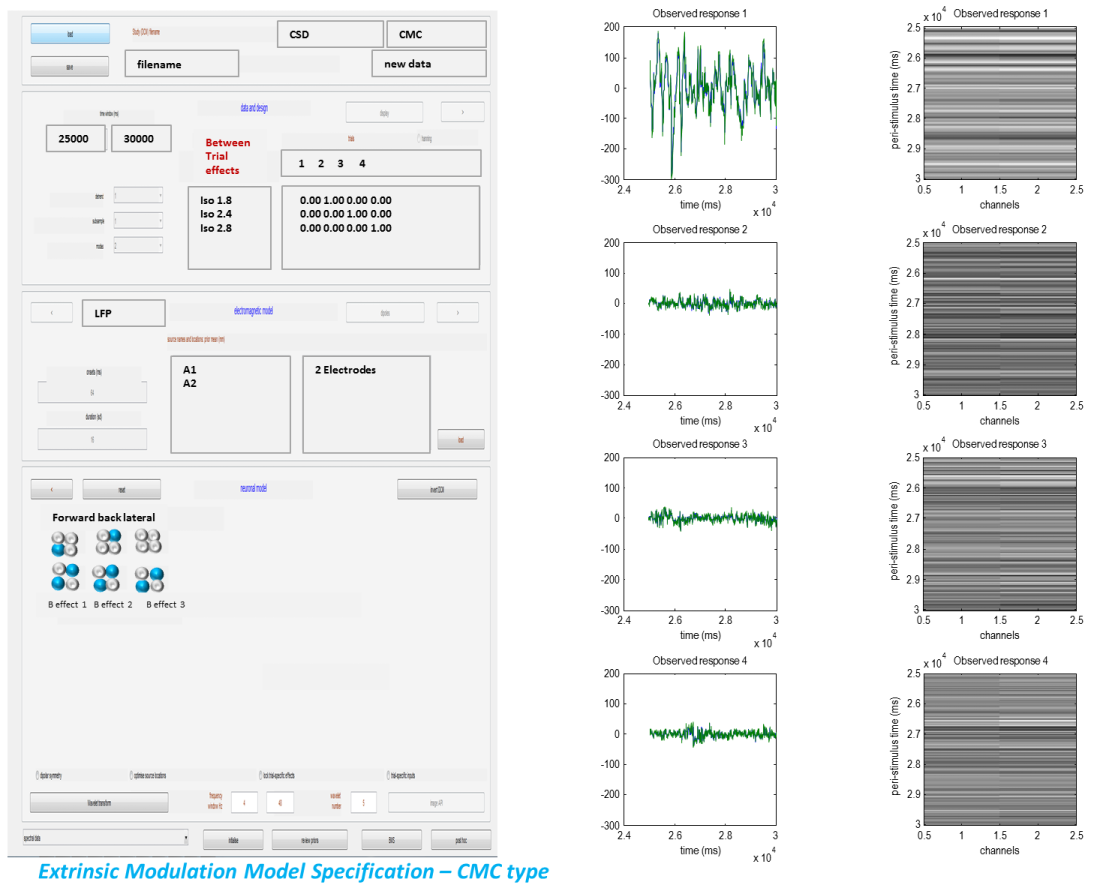
\includegraphics[width=140mm]{dcm_csd/dcm_csd_fig1}
\caption{\em Left: Graphical User Interface to specify model 1: An extrinsic modulation by Isolurance. Here the B effects are clicked along the off-diagonal positions, representing changes in forward and backward extrinsic connections across the three trial types.
Right: Data time series for two intracranial electrode recordings from 25000 to 30000 msec. Green and Blue lines represent different electrodes, panel rows correspond to the different trials -- here recordings made at different depths of anasthaesia: trial 1 = 1.4\% isoflurane, trial2 = 1.8\%, trial 3 = 2.4\% and trial 4 -2.8\%.  \label{dcm_ssr:fig1}}
\end{center}
\end{figure}

\begin{itemize}
\item Finally we enter the frequencies we are interested in: we will fit frequencies from 4 to 48 Hz. 
\item To invert the model press the ``invert DCM'' button.
\item Repeat the procedure after loading the saved specs and repeating for new neuronal models as per figure~\ref{dcm_ssr:fig2}. Here we enter our alternative hypothesis (model 2) and fit a second model where instead of extrinsic connectivity changes, the isoflurane related-changes are generated by connectivity differences within a region – we call this the intrinsic modulation model.
\item This is specified by selecting the diagonal elements of the B-matrices.
\end{itemize}

\begin{figure}
\begin{center}
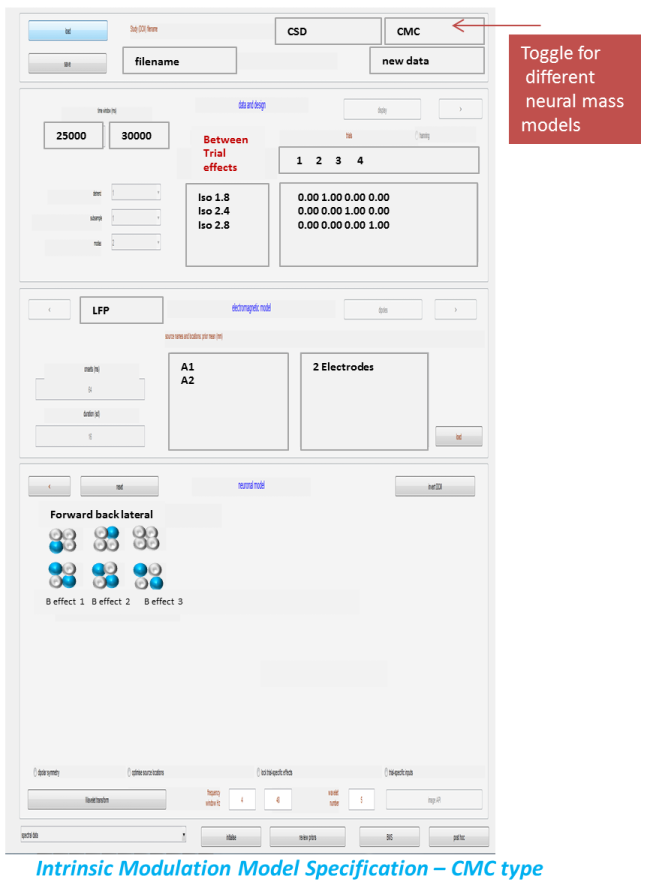
\includegraphics[width=140mm]{dcm_csd/dcm_csd_fig2}
\caption{\em GUI illustrating how to specify model 2 -- the intrinsic modulation model. Here the B effects are clicked along diagonal position, representing changes in local (within-region) coupling. The top panel contains the neural model specification. This can be toggled to select different neural mass models as the basis for the DCM -- eg. LFP or CMC type. 
 \label{dcm_ssr:fig2}}
\end{center}
\end{figure}

\subsection{Comparing models using Bayesian Model Selection}

\begin{itemize}
\item Once both models have run, we compare their evidences to find the best or winning model. 
To do this press the BMS button. This will open the SPM batch tool for model selection. Specify a directory to write the output file to. For the Inference method select Fixed effects (see  \cite{klaas_bms} for additional explanations). Then click on Data and in the box below click on New: Subject. Click on Subject and in the box below on New: Session. Click on models and in the selection window that comes up select the DCM mat files for all the models (remember the order in which you select the files as this is necessary for interpreting the results). Then run the model comparison by pressing the green Run button. You will see at the top, a bar plot of the log-model evidences for all models (Figure~\ref{dcm_ssr:fig3}). The bottom panel displays the conditional probability, for each model assuming equal priors on model space. By convention, a model can be said to be the best among a selection of other models, with strong evidence, if its log-model evidence exceeds all other log-model evidences by at least 3. You can also compare model evidences manually if you load the DCMs into \matlab\ ’s workspace and find the evidence in the structure under DCM.F.
\item For our example we see that there is strong model in favor of model 2 (log Bayes Factor >2500); ie. Isoflorane effects are better explained by a modulation of intrinsic connections.
\item We repeated the steps above and inverted two models (again with either extrinsic or intrinsic modulations) using the CMC and the NMDA neural masses also. These yielded similar results in favor of model 2 – an intrinsic connectivity effect. 
\end{itemize}

\begin{figure}
\begin{center}
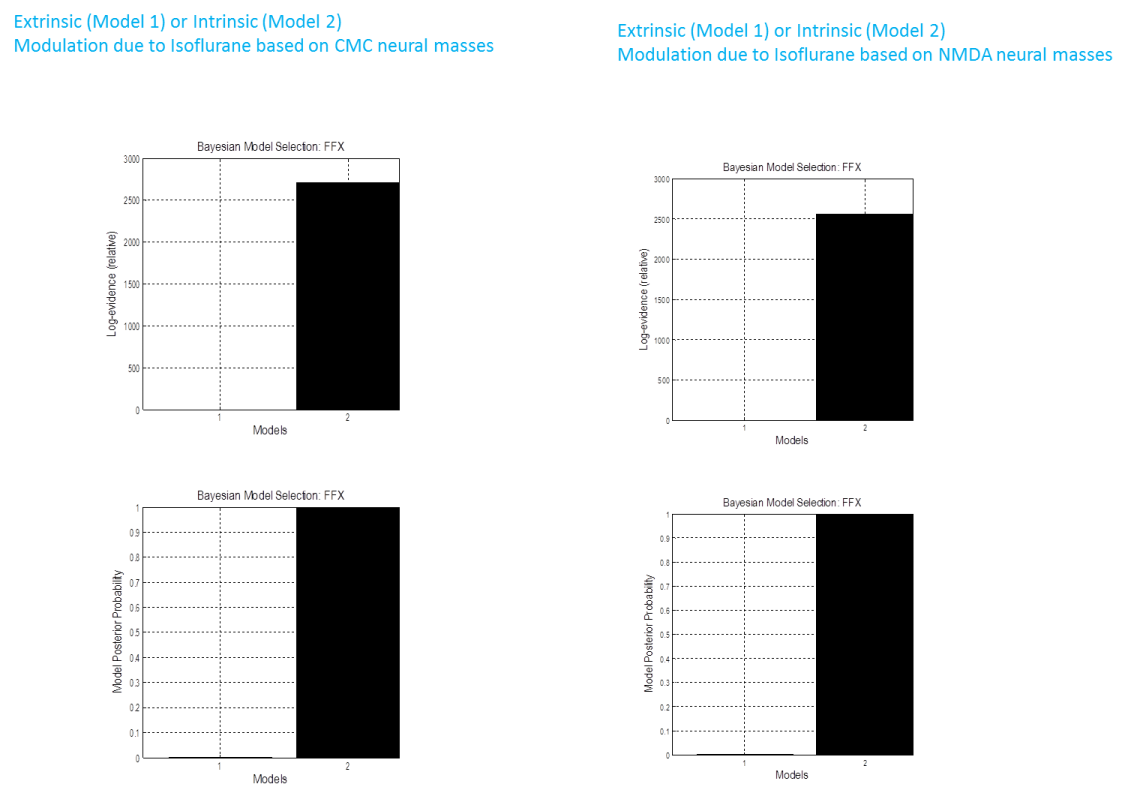
\includegraphics[width=140mm]{dcm_csd/dcm_csd_fig3}
\caption{\em  Top: a bar plot of the log-model evidences for all models. Bottom: conditional probability for each model assuming equal priors on model space. \label{dcm_ssr:fig3}}
\end{center}
\end{figure}

\begin{itemize}
\item Once inverted a results tab appears which allows you to view the fits to the spectral data, posterior parameter estimates, coherence and covariance (in channel and source space) and the transfer functions between regions. You can also examine the direction of the modulating “B” effects under “trial specific effects”.
\item From our winning CMC model we examined the trial specific effects and found a large increase for trial 2 relative to trial 1 in A1 (top left panel). Remember for the CMC case this represents a decreases in pyramidal cell gain – and so is a net inhibitory effect, consistent with the physiological effects of Isoflurane. The effect was even larger for trial 3 compared to trial 1 and decreased to a lower level for trial 4 (as reported in \cite{rm_massmodelspectral}). The effects were similar in A2 (bottom right panel). We found a very similar trial specific effect in the NMDA case, but here the parameter decreases as it represents a positive modulation of an excitatory connection. In other words the effect of increasing isoflurane levels inhibitory in a non-linear fashion (saturating at a level of 2.4\%; trial 3).
\end{itemize}

\begin{figure}
\begin{center}
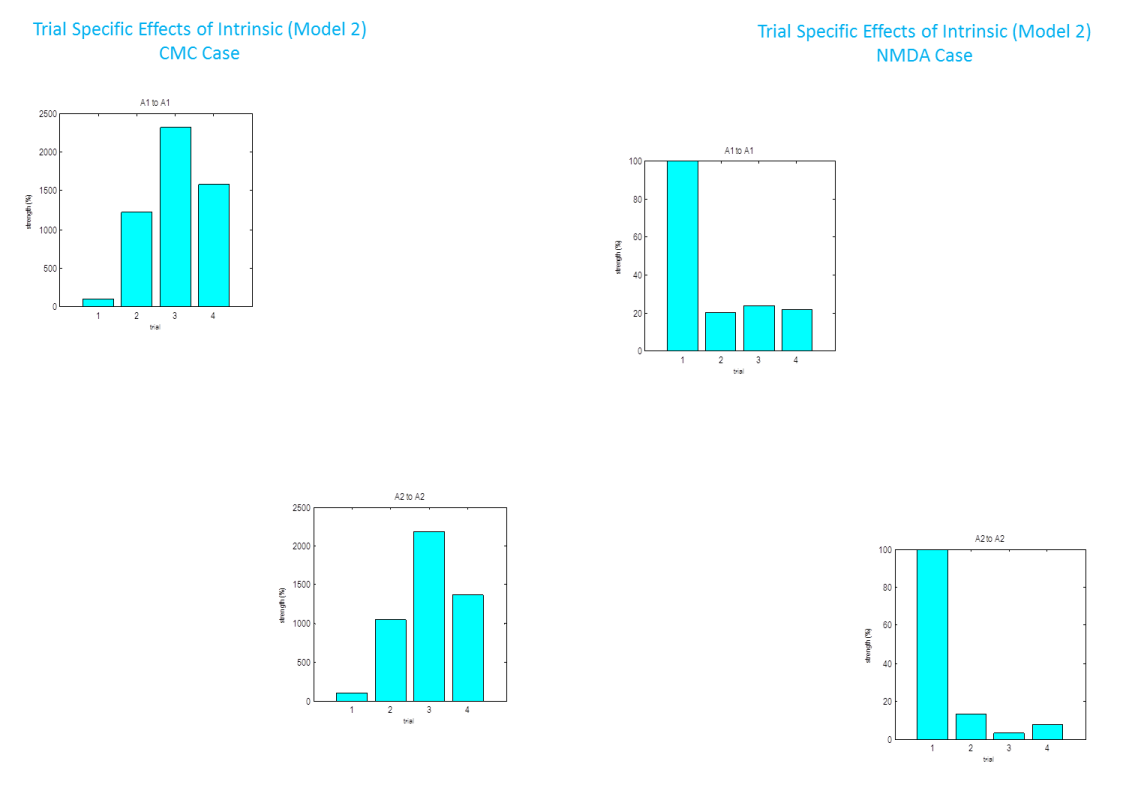
\includegraphics[width=140mm]{dcm_csd/dcm_csd_fig4}
\caption{\em  \label{dcm_ssr:fig4}}
\end{center}
\end{figure}
